\section{Introduction}
Breakout is an arcade game that was published and developed by Atari, where the player is in control of a paddle on the \(x\)-axis and tries to break down each brick by handling a ball. At each time the ball touches to a brick, that particular brick is destroyed and the player gains a point, the game is won if all the bricks are destroyed. A sample position from the game is provided in~\autoref{fig:breakout_image}.

\begin{figure}[h]
    \centering{}
    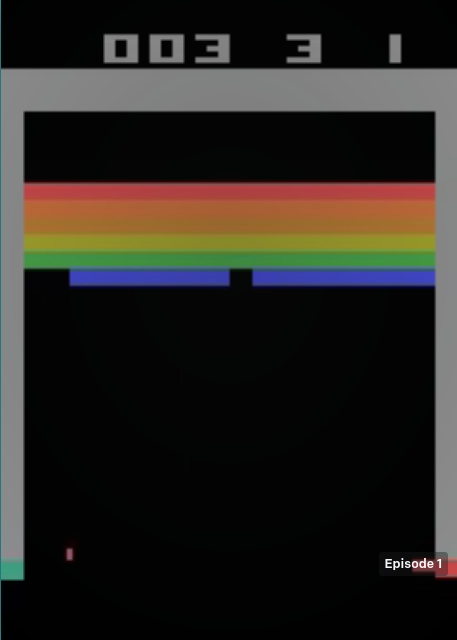
\includegraphics[width=\linewidth, height=0.33\textheight, keepaspectratio]{img/breakout.png}
    \caption{Sample Position from the Breakout Atari Game~\autocite{breakout_image}}~\label{fig:breakout_image}
\end{figure}

In order to obtain a model that can play the game and get better results than a random agent with the use of Supervised or Unsupervised Learning, a large amount of data needs to be generated. Reinforcement learning doesn't need any
data. In reinforcement learning, an agent who has a set of actions is trained in an environment using rewards or punishments considering the decisions of the agent in different situations.

In reinforcement learning, there is a \emph{environment}, which have different states changes at each time step, \(s_t \in S\), and a learning \emph{agent} who can observe the environment and then learns from the outcomes of it's actions, \(a_t \in A\). In reinforcement learning problems, the agents' decisions influence their own actions in proceeding steps, agents don't have any information of which actions to take in what situation and they try to maximize reward (or minimize punishment) by trying out different combinations in the set of actions.

One of the main challenges of RL is to build a model that can learn from the noisy and delayed environmental data. The latency between the incoming data forces training model to give a delayed input reaction and the delays add up to each other in a cascading manner. To overcome the delay problem significantly, rather than using computer vision to gather frames and analyze them one by one, a breakout game developed in such a way that all in-game data can be accessible to the model.

Another challenge is the incoming state data being highly correlated with the previously acquired ones, rather than being independent. To build a model which can perform well withing the high-dimensional correlated state space, a Deep Q-Network (DQN) is developed which combines reinforcement learning with deep neural networks. The many layered approach made it possible to build up more abstract representations of the correlated spatial data.

To be able to train our model, the action set, state space and rewards were defined for the Breakout game. The positive reward are defined as unit positive reward for every break of a brick. No negative rewards are defined. However, in order to stop the repetitive behavior, such as bouncing the ball of the wall and getting it back without breaking any bricks and exploiting the positive rewards, a random restart protocol is implemented, so that the model is pushed to explore rather than exploit.